\chapter{Apresentação dos Resultados}

Nesta seção estão apresentados os resultados obtidos em relação à arquitetura, documentação, testes, usabilidade e
validação dos resultados entregues pela ferramenta.
Para realizar a validação dos resultados, foram feitas comparações com casos da bibliografia, com dados de experimentos
práticos já realizados e também a aplicação em um sistema real.


\section{Arquitetura}
Com o Desenvolvimento do projeto a arquitetura geral das classes se manteve.
Contudo, os métodos já existentes foram melhor definidos, além de serem adicionados diversos outros.
A estrutura geral do diagrama pode ser visualizada na figura \ref{fig:class_diag_new} e os detalhes nas figuras
\ref{fig:class_diag_diubmi_new}, \ref{fig:class_diag_du_new}, \ref{fig:class_diag_pu_new},
\ref{fig:class_diag_model_new}, \ref{fig:class_diag_controller_new} e \ref{fig:class_diag_bcacontroller_new} .

\begin{figure}[H]
    \centering
    \caption{Novo diagrama de classes}
    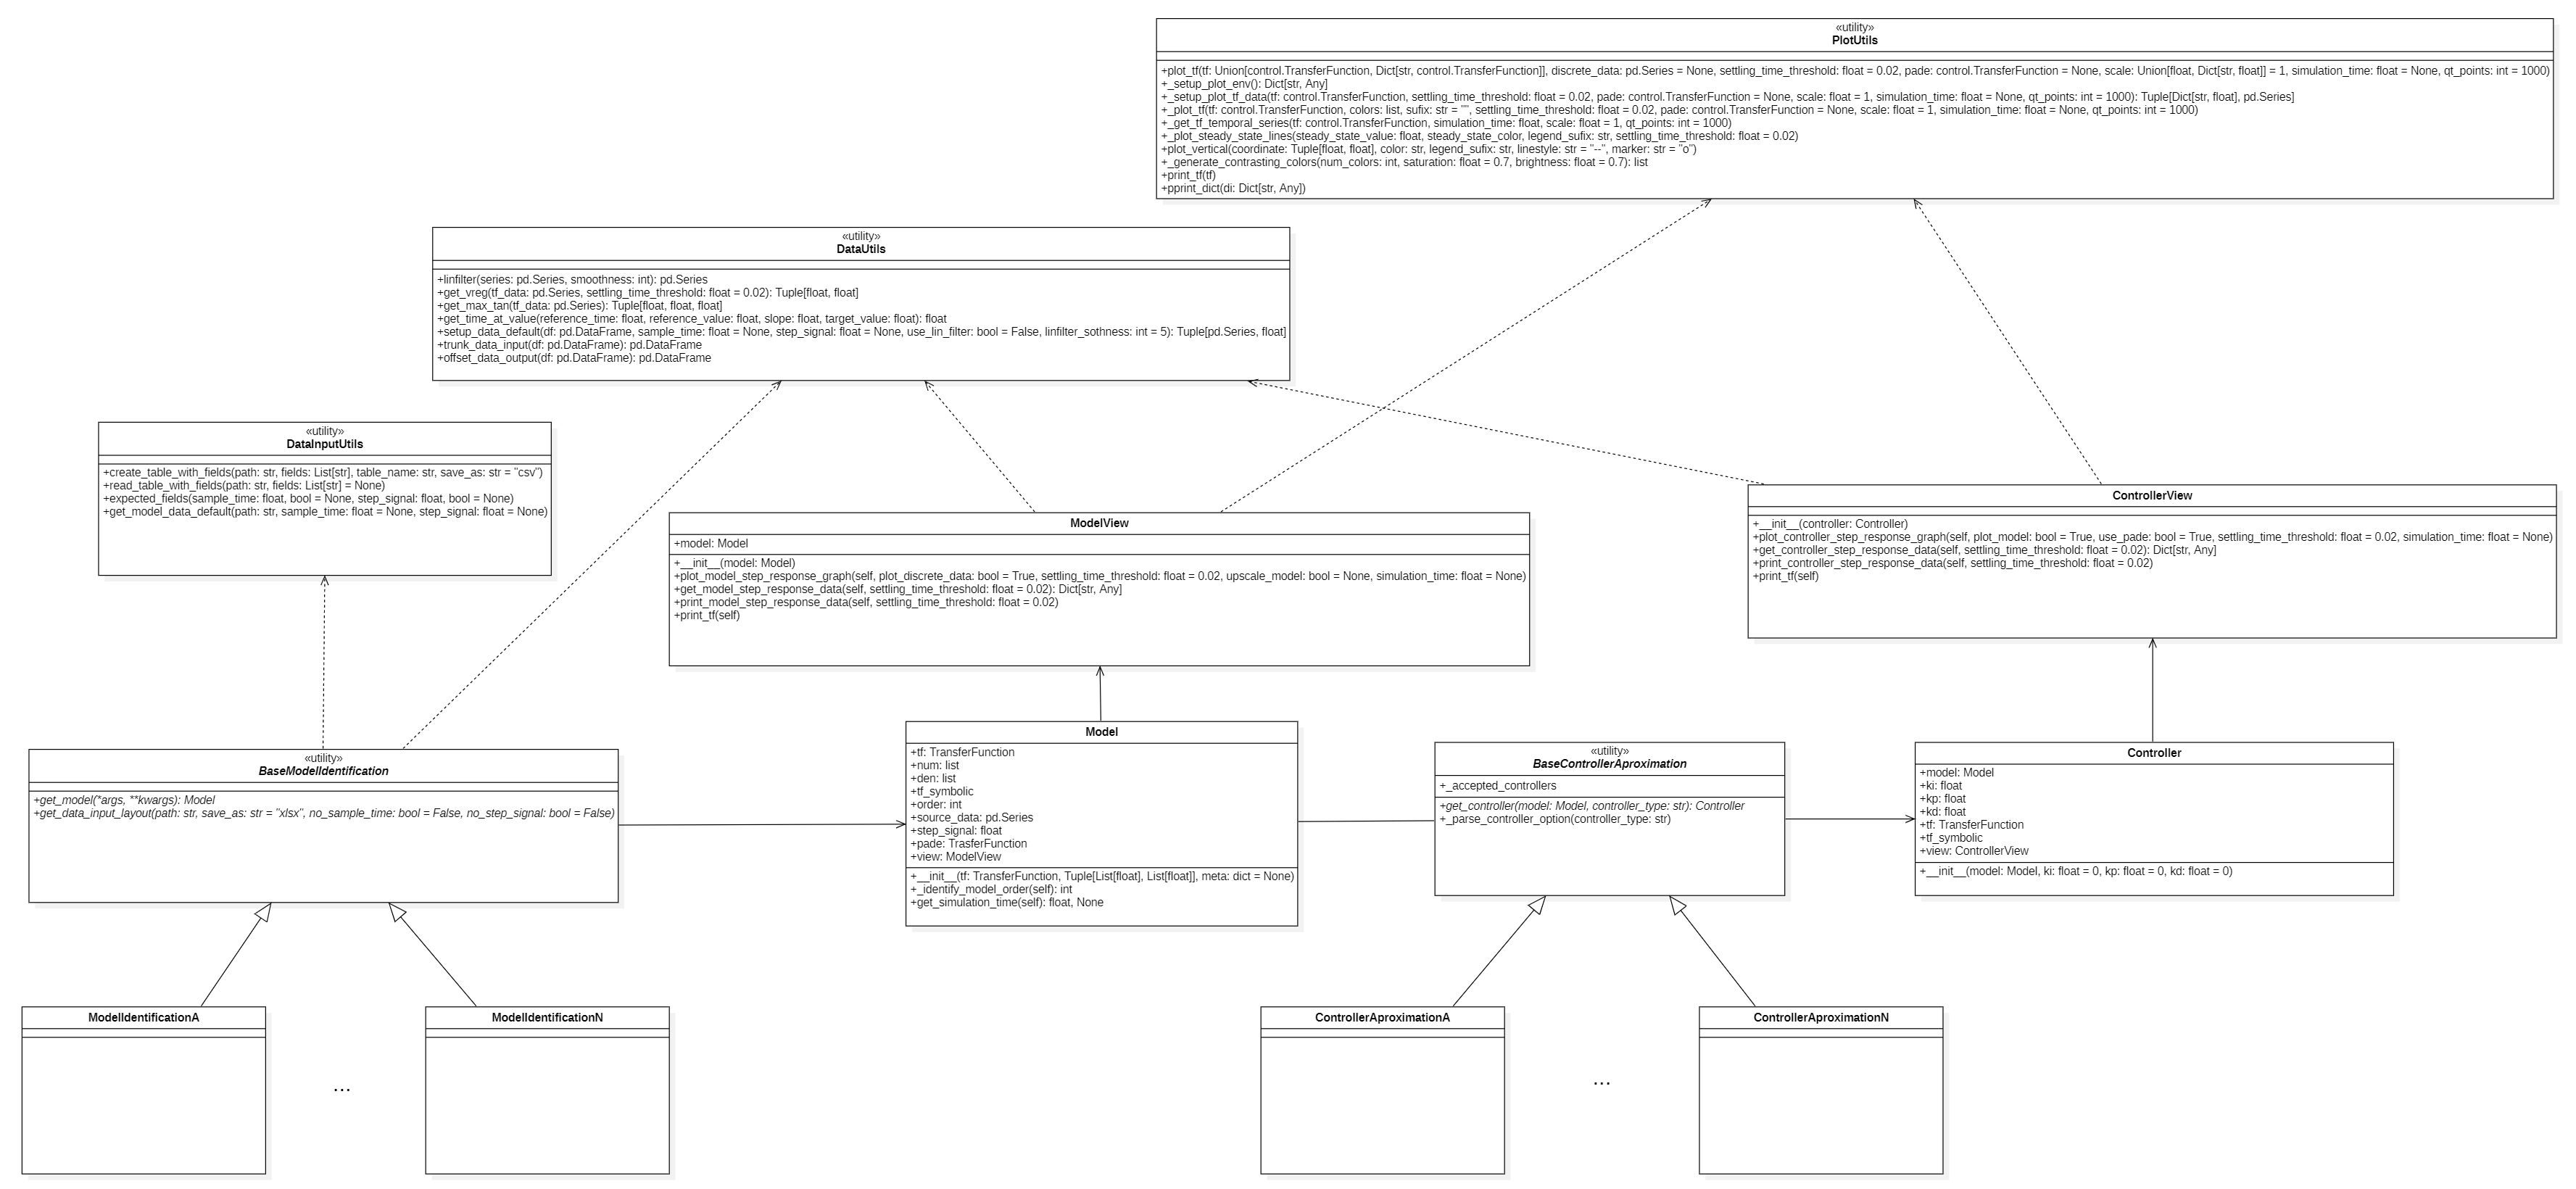
\includegraphics[scale=0.17]{figuras/class_diag_new}
    \label{fig:class_diag_new}
    \\
    \vspace{0cm}\hspace{0cm}\small{Fonte: Do autor}
\end{figure}

\begin{figure}[H]
    \centering
    \caption{Novo diagrama de classes ampliado - DataInputUtils e BaseModelIdentification}
    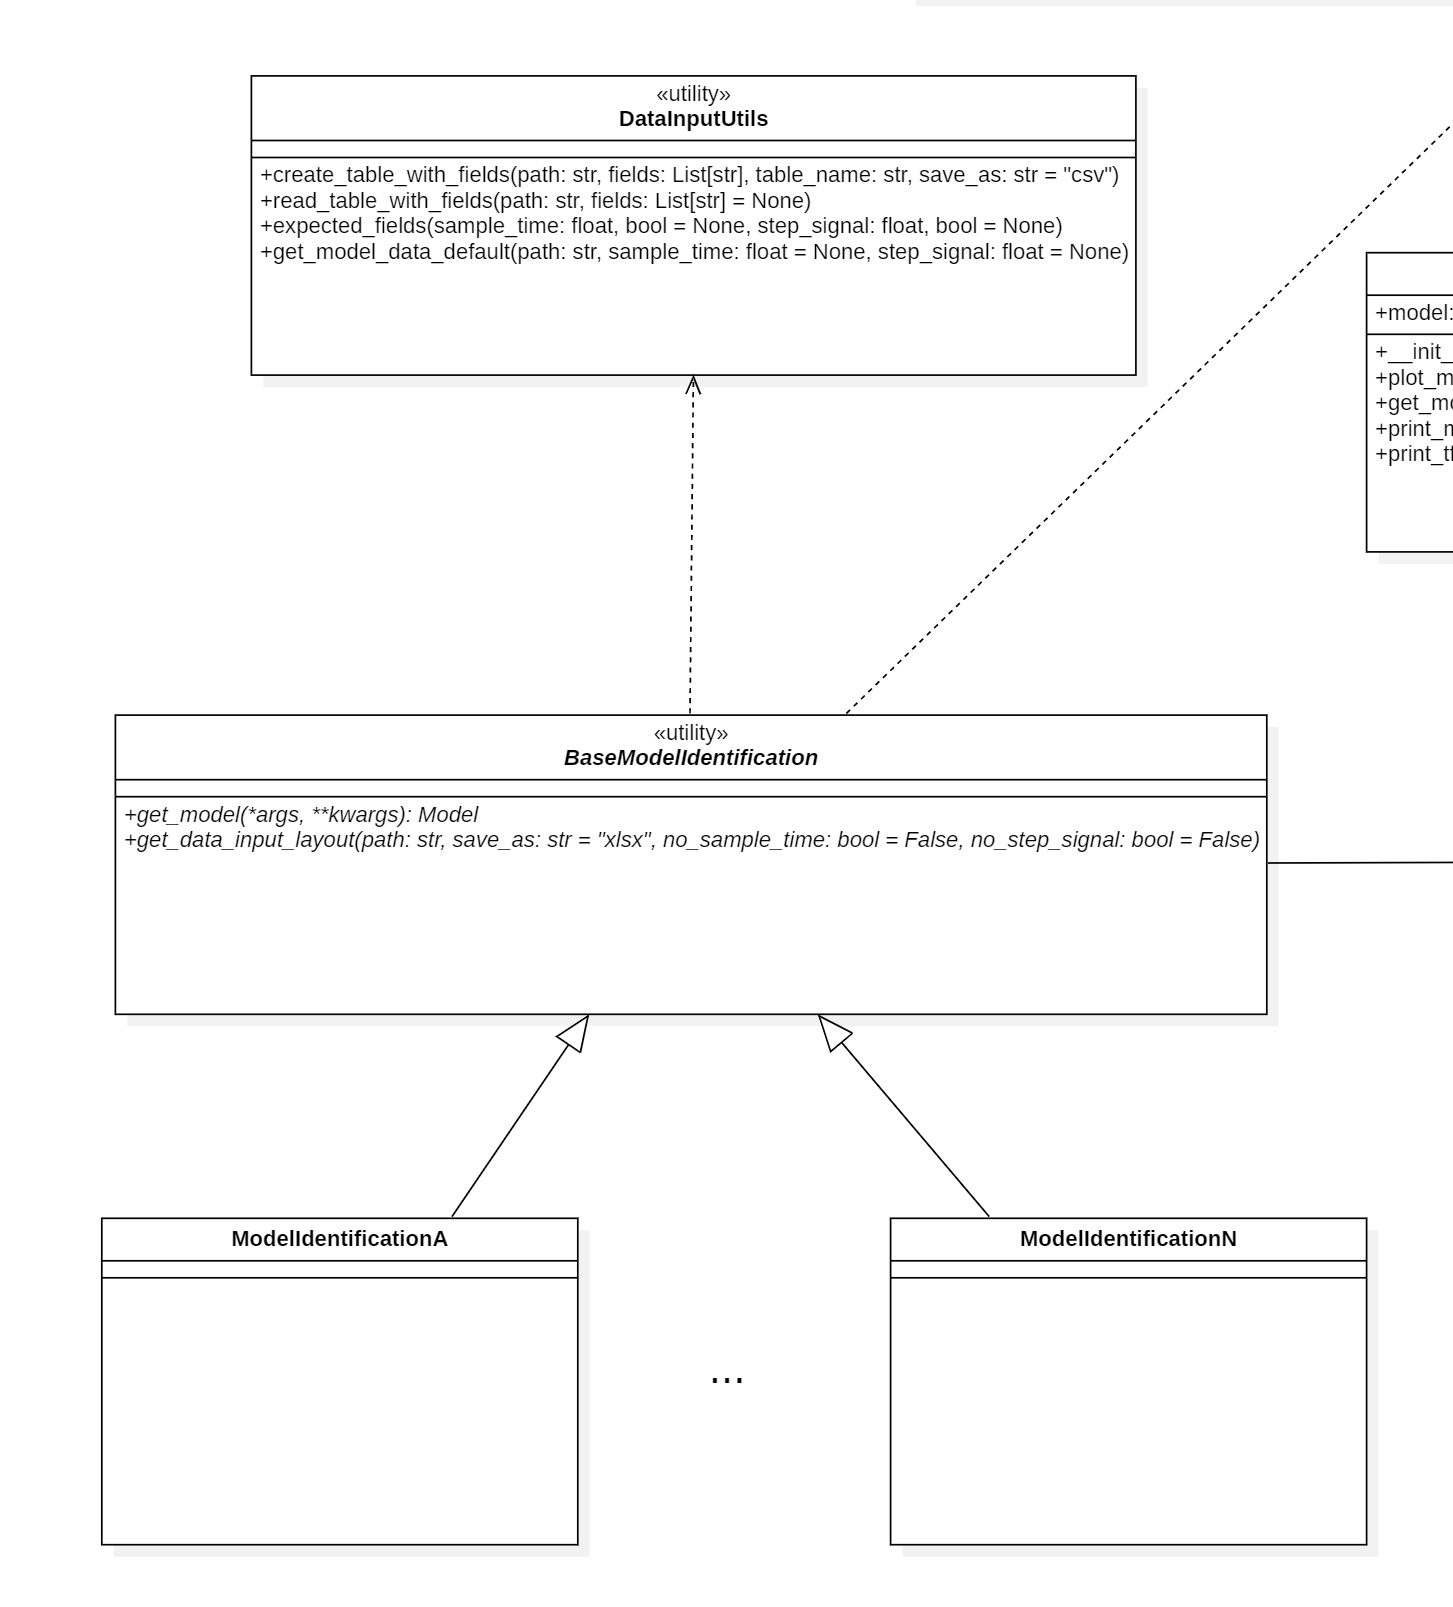
\includegraphics[scale=0.35]{figuras/class_diag_diubmi_new}
    \label{fig:class_diag_diubmi_new}
    \\
    \vspace{0cm}\hspace{0cm}\small{Fonte: Do autor}
\end{figure}

\begin{figure}[H]
    \centering
    \caption{Novo diagrama de classes ampliado - DataUtils e PlotUtils}
    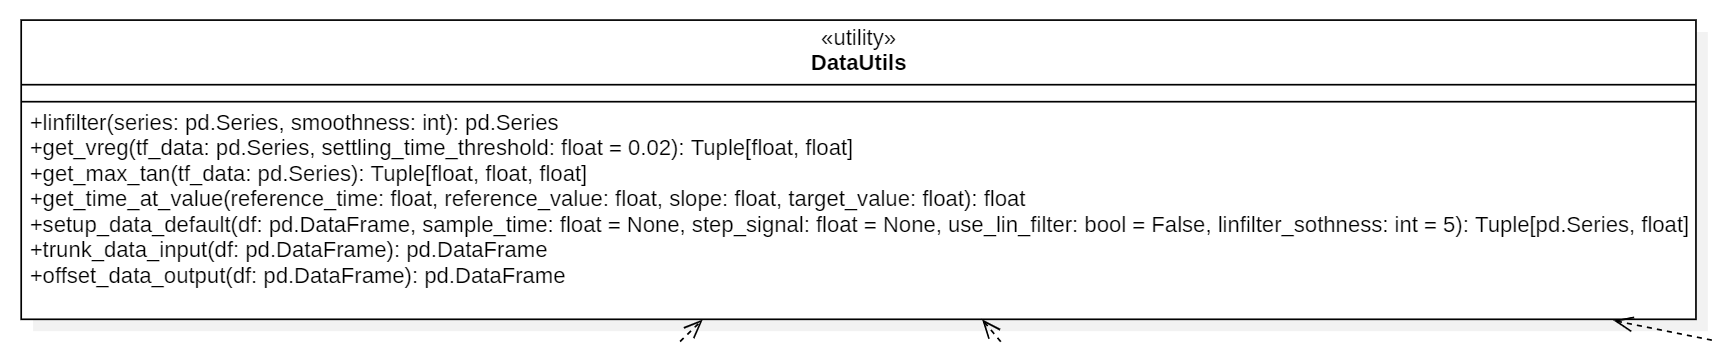
\includegraphics[scale=0.35]{figuras/class_diag_du_new}
    \label{fig:class_diag_du_new}
    \\
    \vspace{0cm}\hspace{0cm}\small{Fonte: Do autor}
\end{figure}

\begin{figure}[H]
    \centering
    \caption{Novo diagrama de classes ampliado - DataUtils e PlotUtils}
    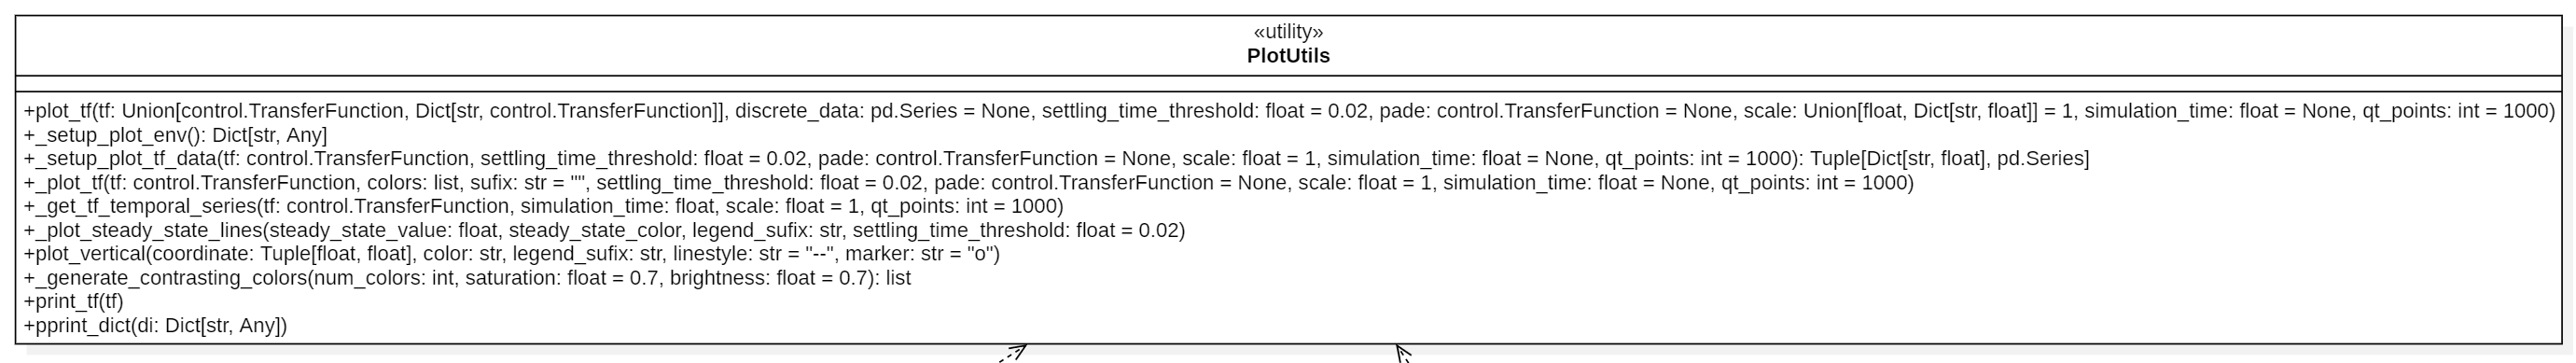
\includegraphics[scale=0.22]{figuras/class_diag_pu_new}
    \label{fig:class_diag_pu_new}
    \\
    \vspace{0cm}\hspace{0cm}\small{Fonte: Do autor}
\end{figure}

\begin{figure}[H]
    \centering
    \caption{Novo diagrama de classes ampliado - Model e ModelView}
    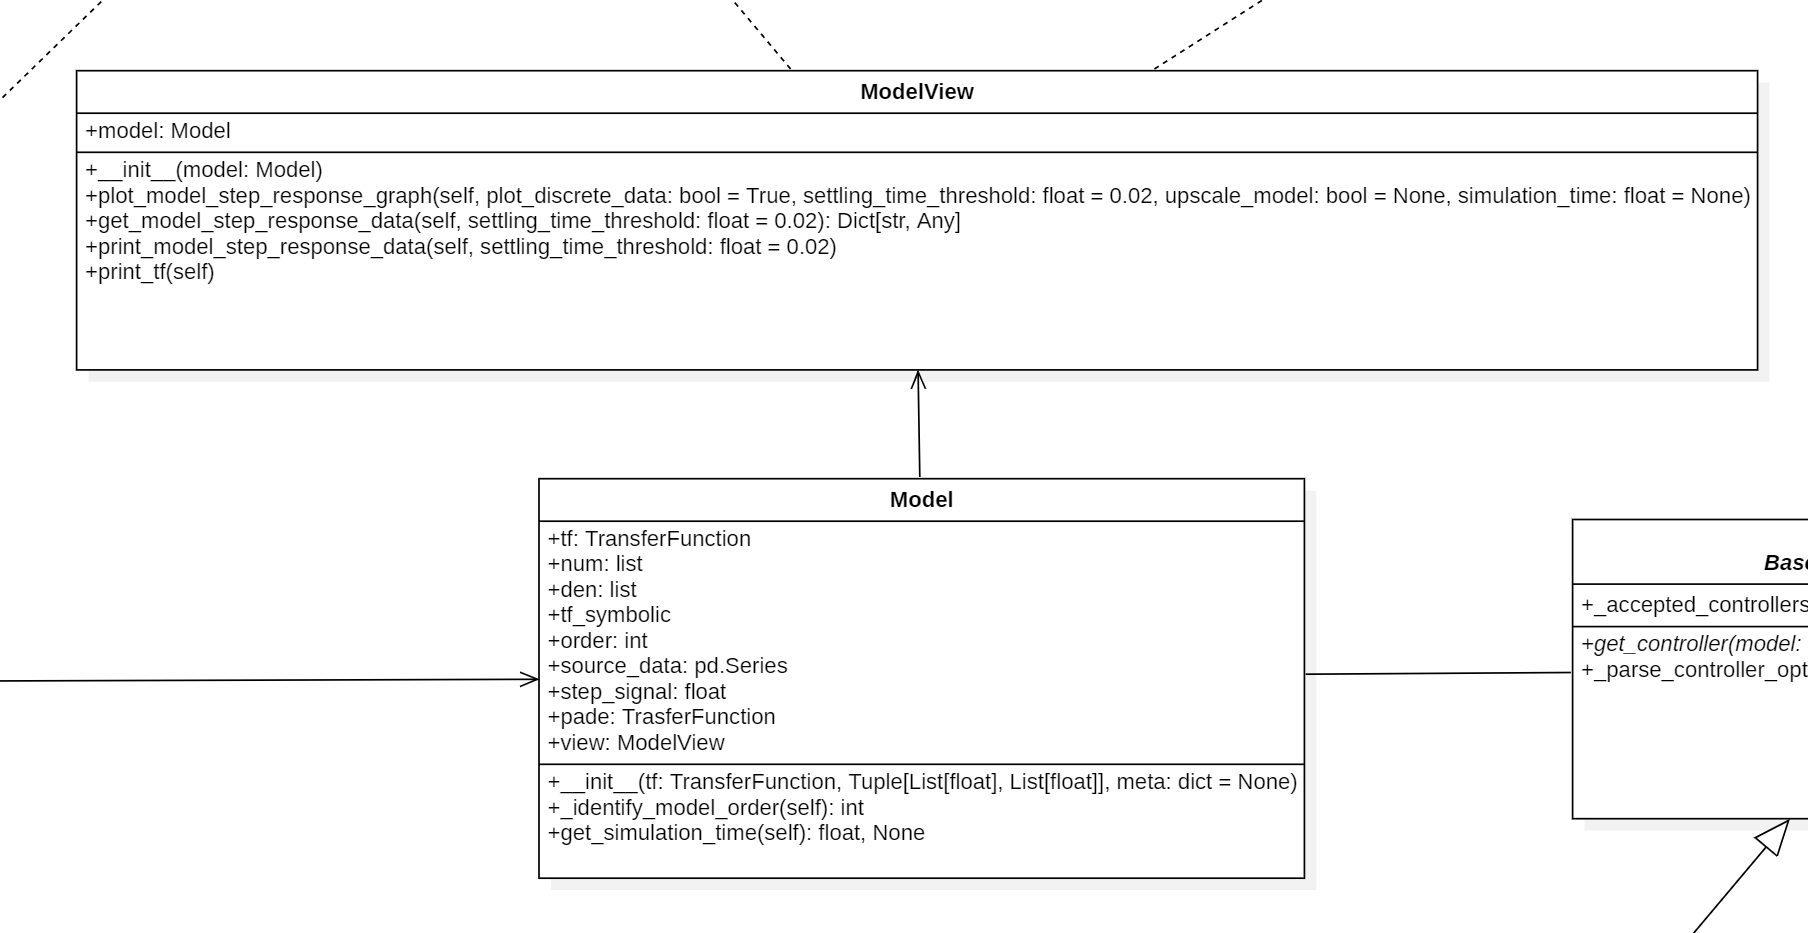
\includegraphics[scale=0.32]{figuras/class_diag_model_new}
    \label{fig:class_diag_model_new}
    \\
    \vspace{0cm}\hspace{0cm}\small{Fonte: Do autor}
\end{figure}

\begin{figure}[H]
    \centering
    \caption{Novo diagrama de classes ampliado - Controller e ControllerView}
    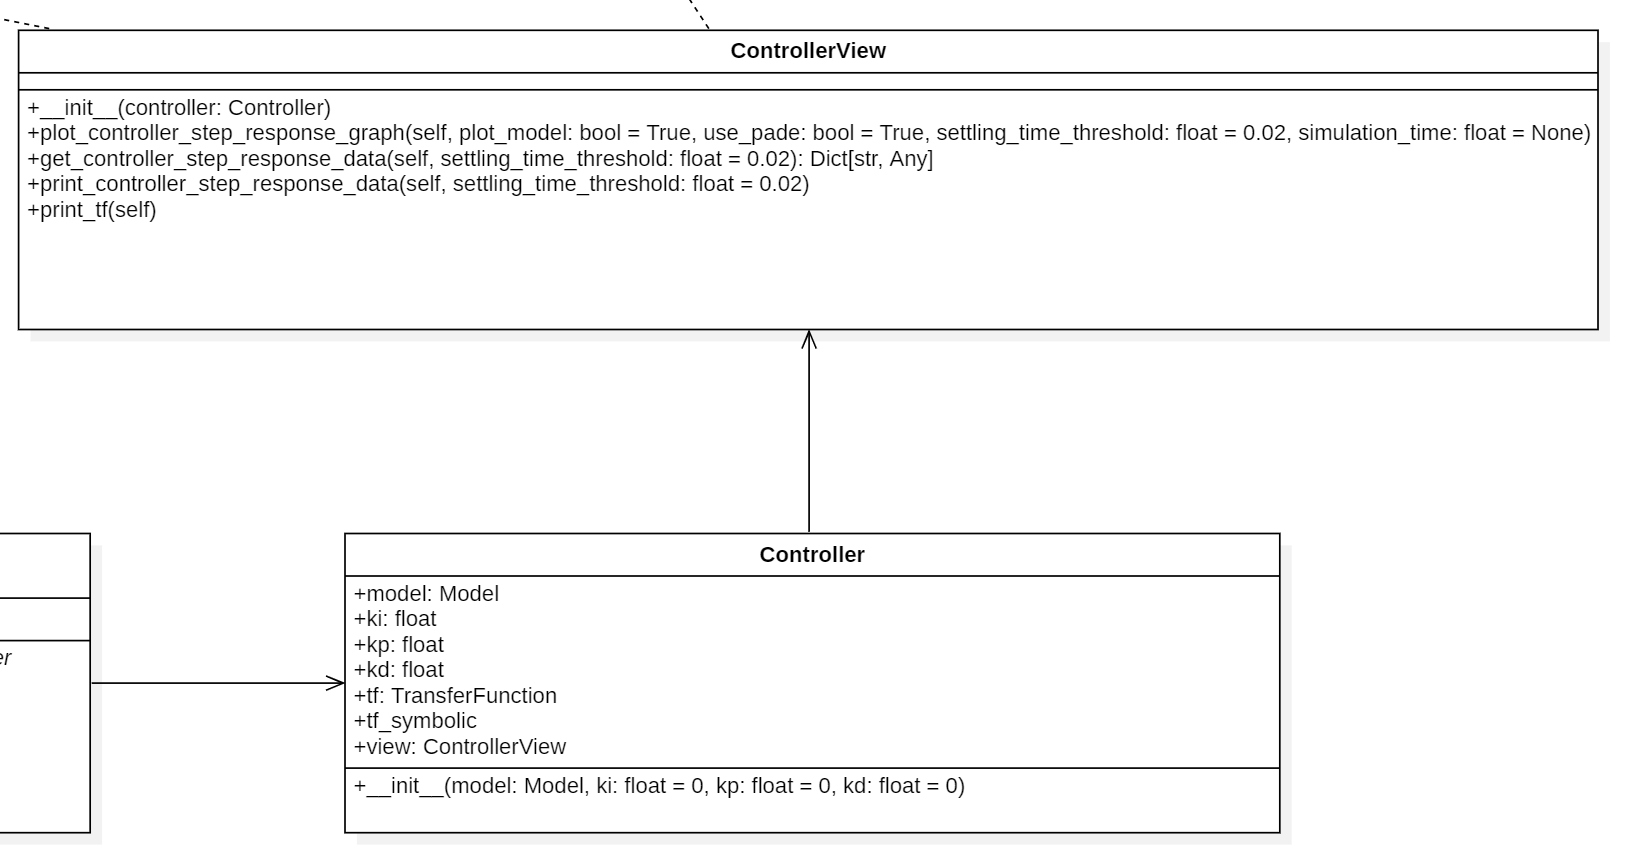
\includegraphics[scale=0.35]{figuras/class_diag_controller_new}
    \label{fig:class_diag_controller_new}
    \\
    \vspace{0cm}\hspace{0cm}\small{Fonte: Do autor}
\end{figure}

\begin{figure}[H]
    \centering
    \caption{Novo diagrama de classes ampliado - BaseControllerAproximation}
    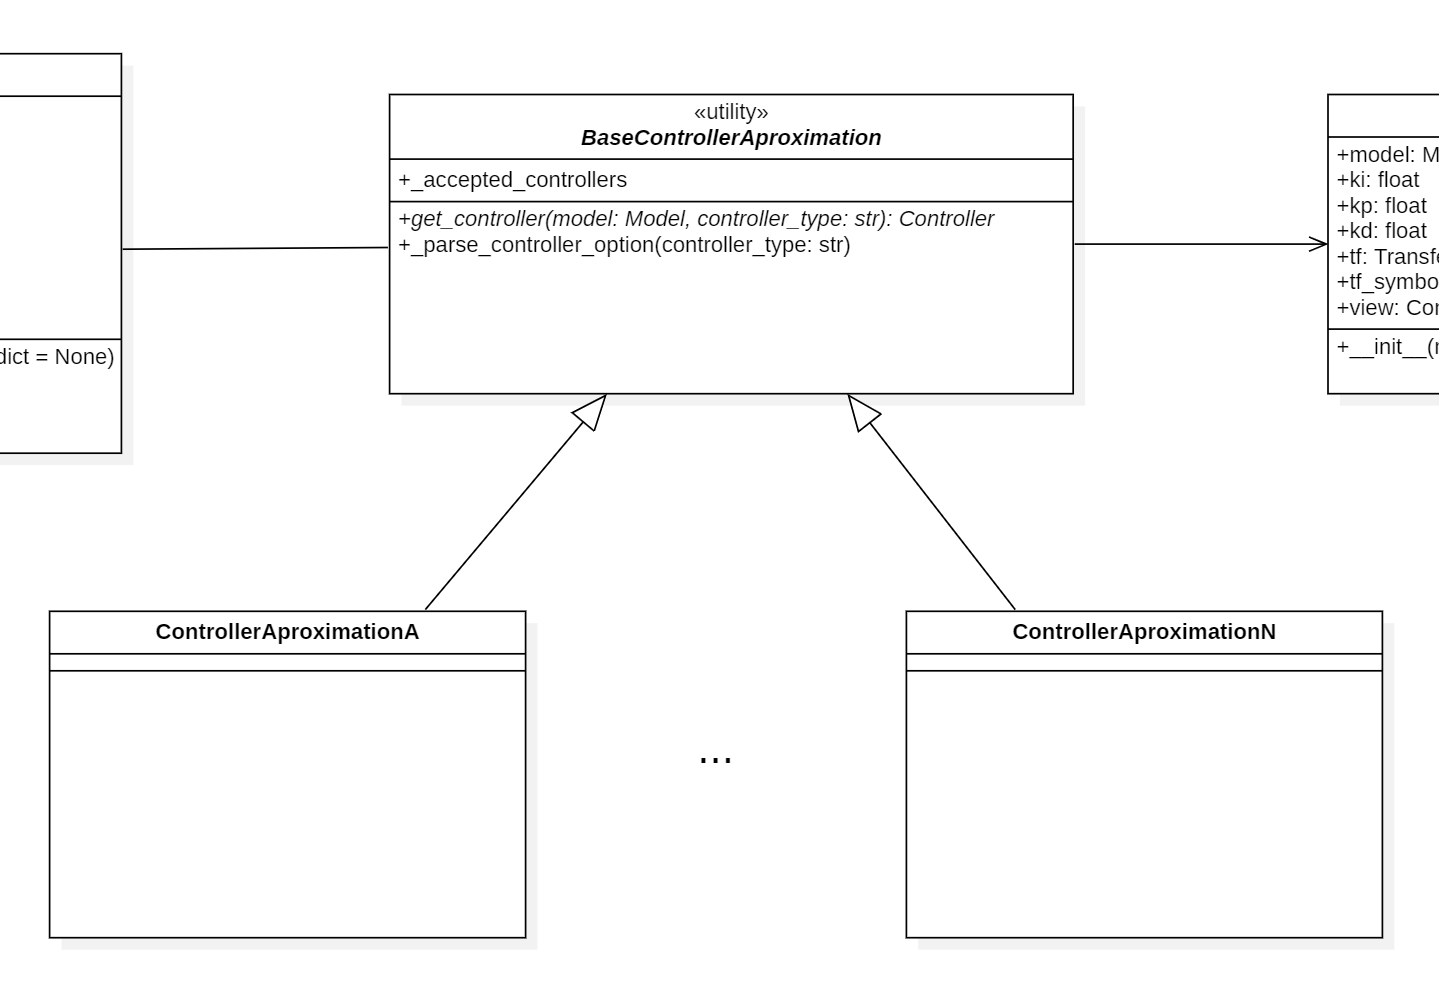
\includegraphics[scale=0.40]{figuras/class_diag_bcacontroller_new}
    \label{fig:class_diag_bcacontroller_new}
    \\
    \vspace{0cm}\hspace{0cm}\small{Fonte: Do autor}
\end{figure}


\section{Documentação}

A documentação desenvolvida juntamente a biblioteca foi compilada com sucesso e disponibilizada no link apresentado
no apêndice \ref{ch:actdocs}.
Ela abrange todas as classes implementadas bem como uma visão ampla da biblioteca e um guia rápido, além de possuir
explicações didáticas sobre o funcionamento de cada método implementado com referências bibliográficas.

TODO: adicionar figura de sumário e explicação mais detalhada de cada página dedicada que foi criada


\section{Testes}

Foi realizado o desenvolvimento de testes para a maioria das funcionalidades da biblioteca, ajudando na detecção
rápida de novos bugs e facilitando futuras implementações.
Uma boa parte do código desenvolvido foi coberto por esses testes, como pode ser visto na figura \ref{fig:coverage}.

\begin{figure}[H]
    \centering
    \caption{Visualização do relatório de cobertura}
    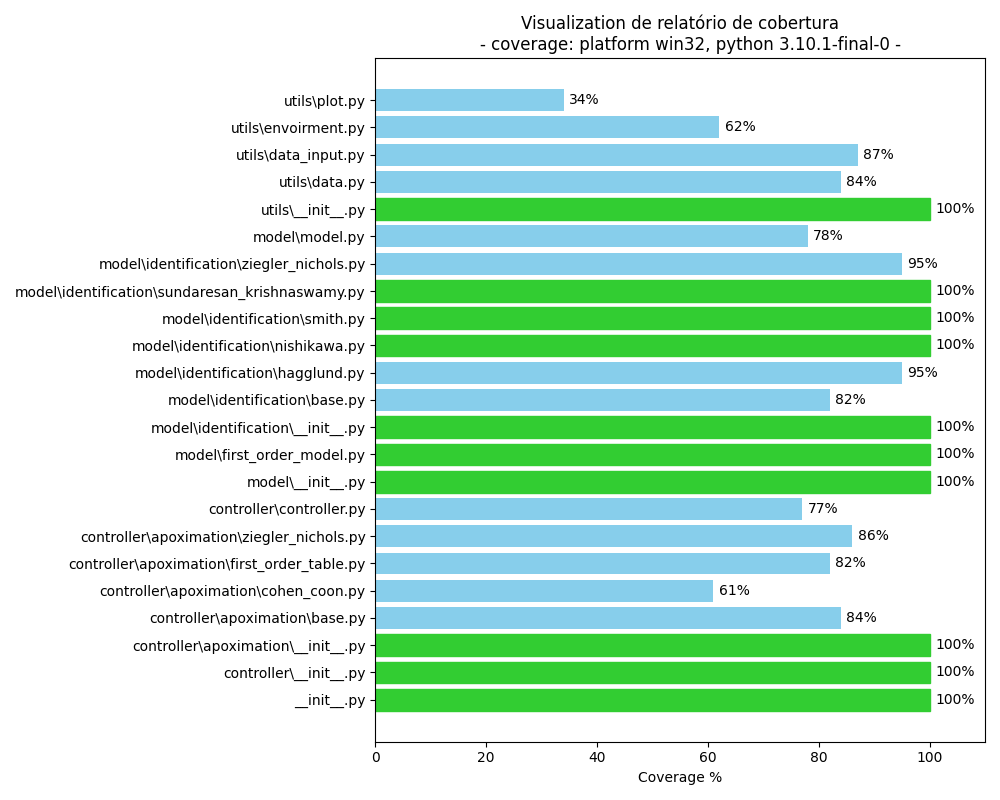
\includegraphics[scale=0.6]{figuras/coverage}
    \label{fig:coverage}
    \\
    \vspace{0cm}\hspace{0cm}\small{Fonte: Do autor}
\end{figure}


\section{Usabilidade}

A biblioteca foi projetada para um uso ágil e simples, de forma que com poucas linhas de código é possível realizar a
identificação de um modelo e a aproximação de ganhos de um controlador, bem como obter informações de suas respostas
a sinal degrau e gráficos para visualização.

Para um caso onde se deseja identificar o modelo de uma planta através do método de Nishikawa e obter um controlador
pelo método de Cohen e Coon, o primeiro paço é importar a biblioteca e obter o leiaute para entrada dos dados:

\begin{lstlisting}[label={lst:get_dil}]
import auto_control_tools as act

act.NishikawaModelIdentification.get_data_input_layout('./', save_as='csv', no_sample_time=True)
\end{lstlisting}

Com isso um arquivo \("\)data\_input.csv\("\) será criado no diretório atual.
Os dados de resposta do sistema devem ser inseridos nele, nesse caso no formato CSV, com os dados separados por vírgula.
O parâmetro no\_sample\_time foi marcado como verdadeiro, indicando para o método de criação do leiaute que não
se deseja informar os dados de tempo de aquisição na planilha fornecida.
Esse dado pode ser fornecido posteriormente como uma constante.

Com o arquivo preenchido com os dados de resposta a sinal degrau do sistema, é possível realizar a identificação,
obtendo um modelo do qual já podemos visualizar os dados e o gráfico de forma simples, como pode ser visto no trecho
de código a seguir:

\begin{lstlisting}[label={lst:get_model}]
import auto_control_tools as act

# act.NishikawaModelIdentification.get_data_input_layout('./', save_as='csv', no_sample_time=True)

model = act.NishikawaModelIdentification.get_model('./data_input.csv', sample_time=1, ignore_delay_threshold=0)

model.view.print_tf()
model.view.print_model_step_response_data()
model.view.plot_model_step_response_graph()
\end{lstlisting}

Para os dados fornecidos, a execução do código imprime as seguintes informações no terminal:
\begin{lstlisting}[label={lst:get_model_out}]
0.841304347826087*exp(-2.22428940568476*s)/(7.60658914728682*s + 1.0)
{'Overshoot': 0,
 'Peak': 0.841304292382592,
 'PeakTime': 128.0,
 'RiseTime': 16.726793943383804,
 'SettlingMax': 0.8413043478260871,
 'SettlingMin': 0.7574087299857988,
 'SettlingTime': 32.02106649111257,
 'SteadyStateValue': 0.8413043478260871,
 'Undershoot': 0.6269523372311043}
\end{lstlisting}

Além disso é aberta uma janela interativa, onde pode ser comparado o resultado da identificação com os dados de entrada
como pode ser visto na figura \ref{fig:get_model_plot}.
Nesse caso a resposta do modelo está sendo redimensionada em relação ao valor do setpoint, para ser possível a
comparação com os dados de entrada.

\begin{figure}[H]
    \centering
    \caption{Exemplo de uso da biblioteca - plot\_model\_step\_response\_graph}
    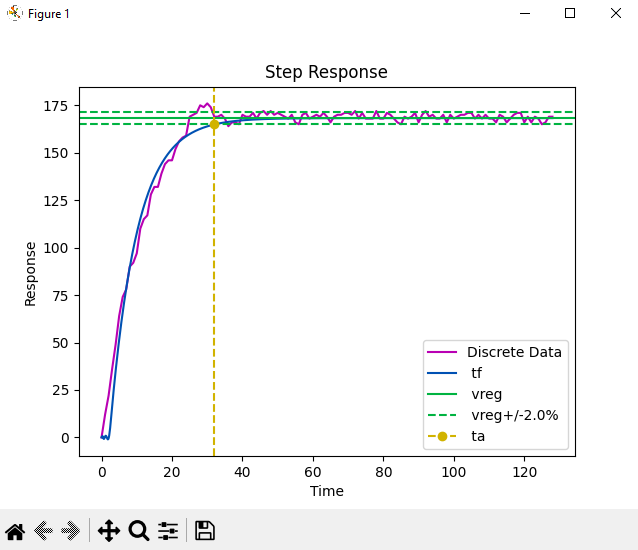
\includegraphics[scale=0.6]{figuras/get_model_plot}
    \label{fig:get_model_plot}
    \\
    \vspace{0cm}\hspace{0cm}\small{Fonte: Do autor}
\end{figure}

O processo de aproximação de ganhos de controlador por Cohen Coon ocorre de forma ainda mais simples, apenas é
necessário fornecer o modelo e o controlador desejado, a etapa de visualização de dados ocorre de forma
idêntica como pode ser visto no trecho de código a seguir:

\begin{lstlisting}[label={lst:get_controller}]
controller = act.CohenCoonControllerAproximation.get_controller(model, act.PID)

controller.view.print_tf()
controller.view.print_controller_step_response_data()
controller.view.plot_controller_step_response_graph()
\end{lstlisting}

Como pode ser visto na sequência, a execução produz uma saida idêntica no terminal, mas agora para o sistema em malha
fechada com o controlador gerado:

\begin{lstlisting}[label={lst:get_controller_out}]
0.841304347826087*(0.768000555728862*s + 5.71697021219369 + 4.89459279701174/s)*exp(-2.22428940568476*s)/((1 + 0.841304347826087*(0.768000555728862*s + 5.71697021219369 + 4.89459279701174/s)*exp(-2.22428940568476*s)/(7.60658914728682*s + 1.0))*(7.60658914728682*s + 1.0))
{'Kd': 0.7680005557288616,
 'Ki': 4.89459279701174,
 'Kp': 5.716970212193688,
 'Overshoot': 22.98302475453806,
 'Peak': 1.2298302475453806,
 'PeakTime': 5.9407504937458855,
 'RiseTime': 1.6853192890059248,
 'SettlingMax': 1.2298302475453806,
 'SettlingMin': 0.9145088850141698,
 'SettlingTime': 12.850559578670177,
 'SteadyStateValue': 1.0,
 'Undershoot': 7.829211261071754}
\end{lstlisting}

O gráfico de resposta plotado por padrão também traz a resposta do modelo em malha aberta para comparação.
Esse comportamento pode ser alterado informando o parâmetro plot\_model como False.
O resultado da plotagem pode ser visto na figura \ref{fig:get_controller_plot}.

\begin{figure}[H]
    \centering
    \caption{Exemplo de uso da biblioteca - plot\_controller\_step\_response\_graph}
    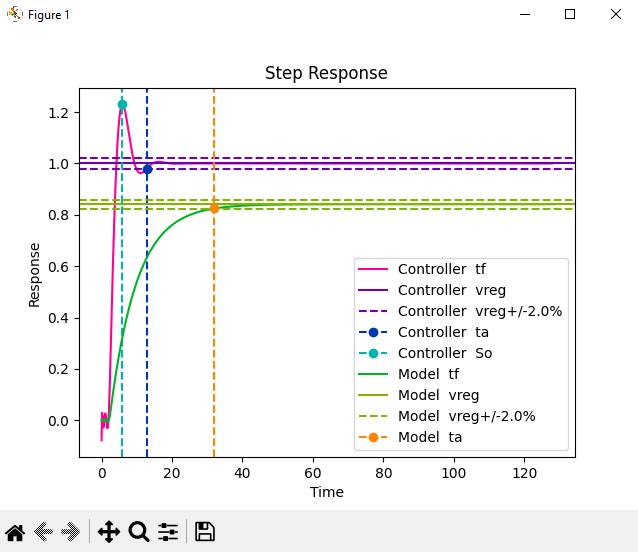
\includegraphics[scale=0.6]{figuras/get_controller_plot}
    \label{fig:get_controller_plot}
    \\
    \vspace{0cm}\hspace{0cm}\small{Fonte: Do autor}
\end{figure}

Adicionalmente, a janela interativa suporta ampliar o gráfico, para melhor visualização da resposta do sistema em
malha fechada, por exemplo.
Uma vista ampliada pode ser observada na figura \ref{fig:get_controller_plot_zoom}.

\begin{figure}[H]
    \centering
    \caption{Exemplo de uso da biblioteca - plot\_controller\_step\_response\_graph - Zoom}
    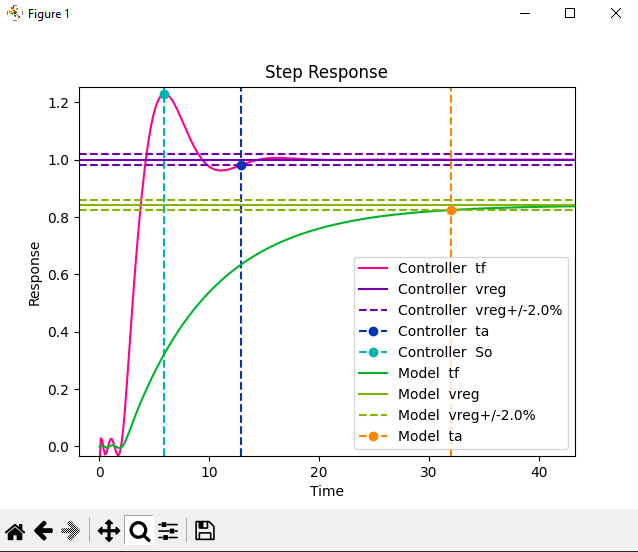
\includegraphics[scale=0.6]{figuras/get_controller_plot_zoom}
    \label{fig:get_controller_plot_zoom}
    \\
    \vspace{0cm}\hspace{0cm}\small{Fonte: Do autor}
\end{figure}

As mesmas operações podem ser executadas em qualquer ambiente com uma versão de Python suportada, inclusive em
ambientes Jupyter.
A seguir, nas figuras \ref{fig:colab_example1}, \ref{fig:colab_example2} e \ref{fig:colab_example3}, é demonstrada a
execução do mesmo código do exemplo anterior, mas desta vez no Google Colab, um serviço gratuito da empresa Google que
permite escrever e executar código Python através do navegador em um ambiente baseado em Jupyter.
Além de estar sendo executado em nuvem, o ambiente baseado em Jupyter possibilita uma formatação mais visualmente
agradável das funções de transferência e das informações de resposta a sinal degrau.

\begin{figure}[H]
    \centering
    \caption{Exemplo de uso da biblioteca - execução no colab - instalação importação e obtenção de leiaute}
    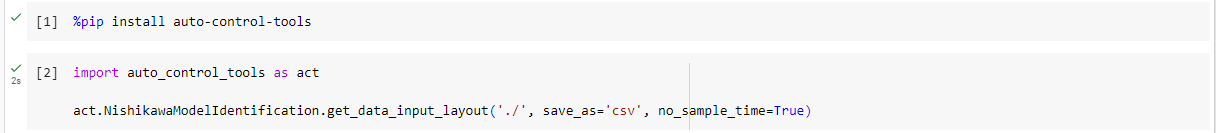
\includegraphics[scale=0.5]{figuras/colab_example1}
    \label{fig:colab_example1}
    \\
    \vspace{0cm}\hspace{0cm}\small{Fonte: Do autor}
\end{figure}

\begin{figure}[H]
    \centering
    \caption{Exemplo de uso da biblioteca - execução no colab - obtenção e visualização de modelo}
    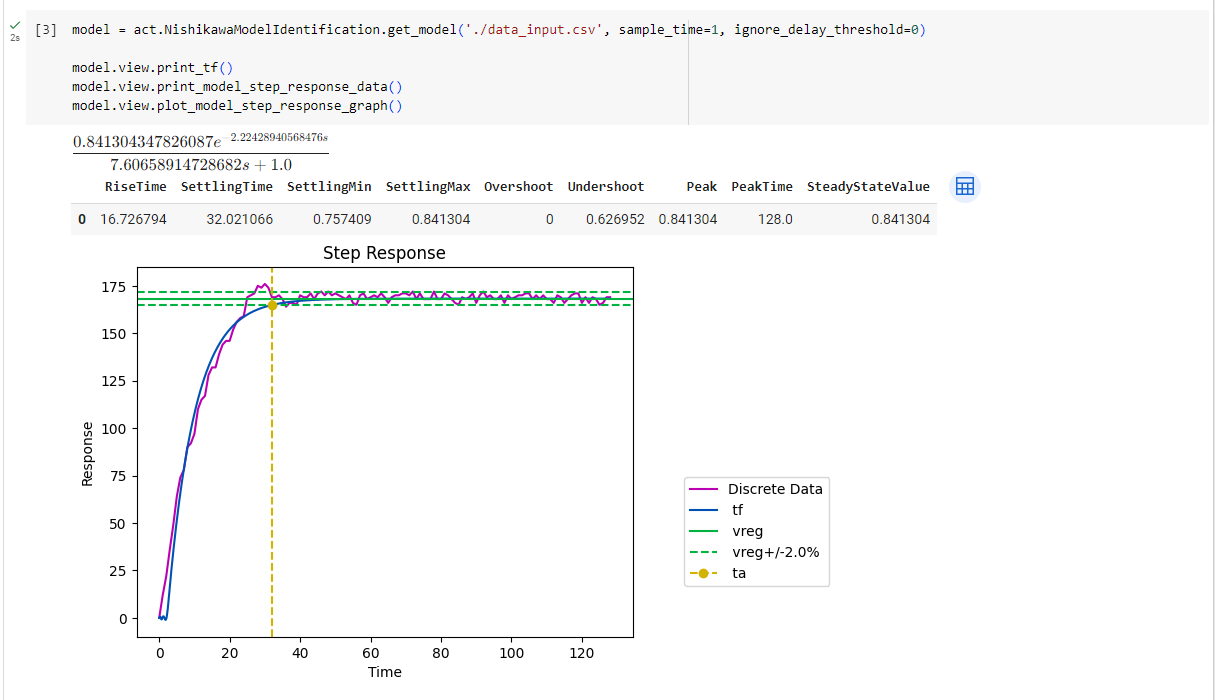
\includegraphics[scale=0.5]{figuras/colab_example2}
    \label{fig:colab_example2}
    \\
    \vspace{0cm}\hspace{0cm}\small{Fonte: Do autor}
\end{figure}

\begin{figure}[H]
    \centering
    \caption{Exemplo de uso da biblioteca - execução no colab - obtenção e visualização de controlador}
    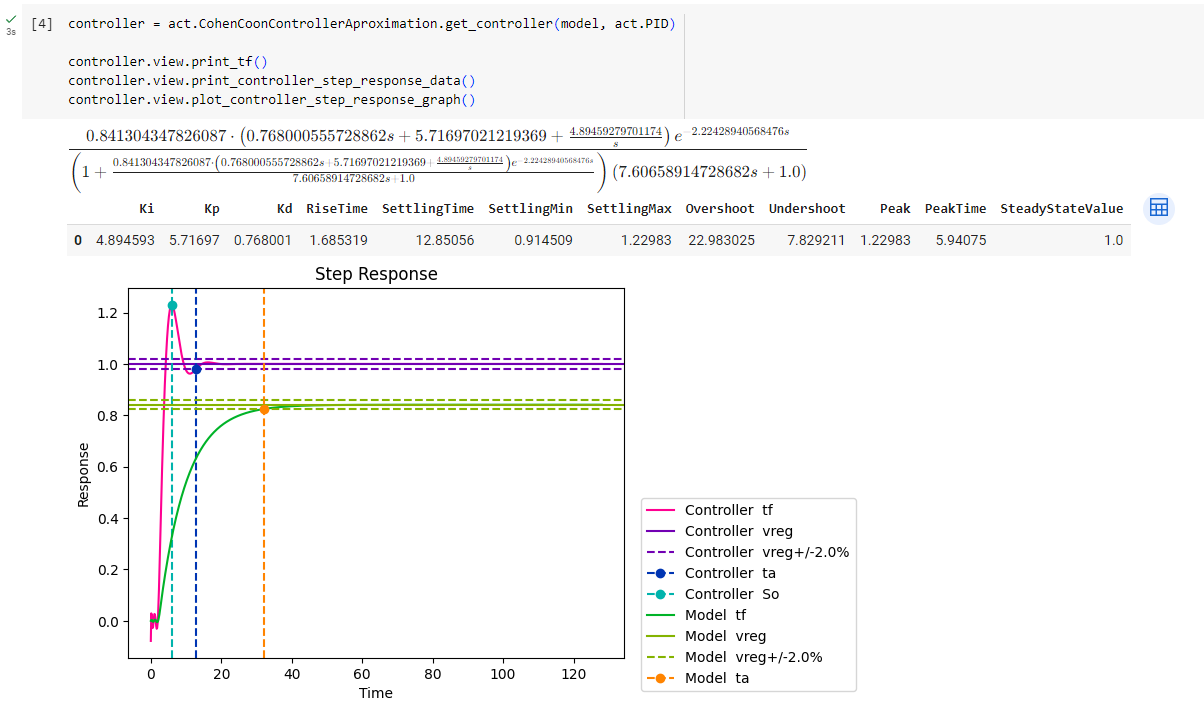
\includegraphics[scale=0.5]{figuras/colab_example3}
    \label{fig:colab_example3}
    \\
    \vspace{0cm}\hspace{0cm}\small{Fonte: Do autor}
\end{figure}


\section{Comparação com a Bibliografia}

As bibliografias de \cite{ogata2010engenharia} e \cite{CoelhoIdentificacao}, a pesar de tratarem de identificação de
modelos, não fornecem dados discretos de resposta a sinal degram para poderem ser comparados aos métodos de
identificação implementados, desta forma esta seção de comparação com a bibliografia tratará apenas dos métodos de
aproximação de ganhos de controladores PID implementados.

\subsection{Biblioteca versus Apostila sobre PID e Métodos de Sintonia}

O primeiro caso a ser explorado será o do exemplo do tanque aquecido de \cite{apostpidsint}.
Nele é apresentado o gráfico da figura \ref{fig:bib_comp_1_graph} e determinados os parâmetros $K$, $\tau$ e $\theta$ para
obtenção do modelo clássico que a classe FirstOrderModel da seção \ref{subsubsec:fom} se especializa.
Os valores calculados podem ser vistos em \ref{eq:bib_comp_1_id} e o modelo obtido é apresentado em
\ref{eq:bib_comp_1_model}.
E os resultados da aproximação de ganhos de controlador obtidos são descritos na tabela \ref{tab:bib_comp_1_restb}.


\begin{figure}[H]
    \centering
    \caption{Curva de reação para o tanque aquecido}
    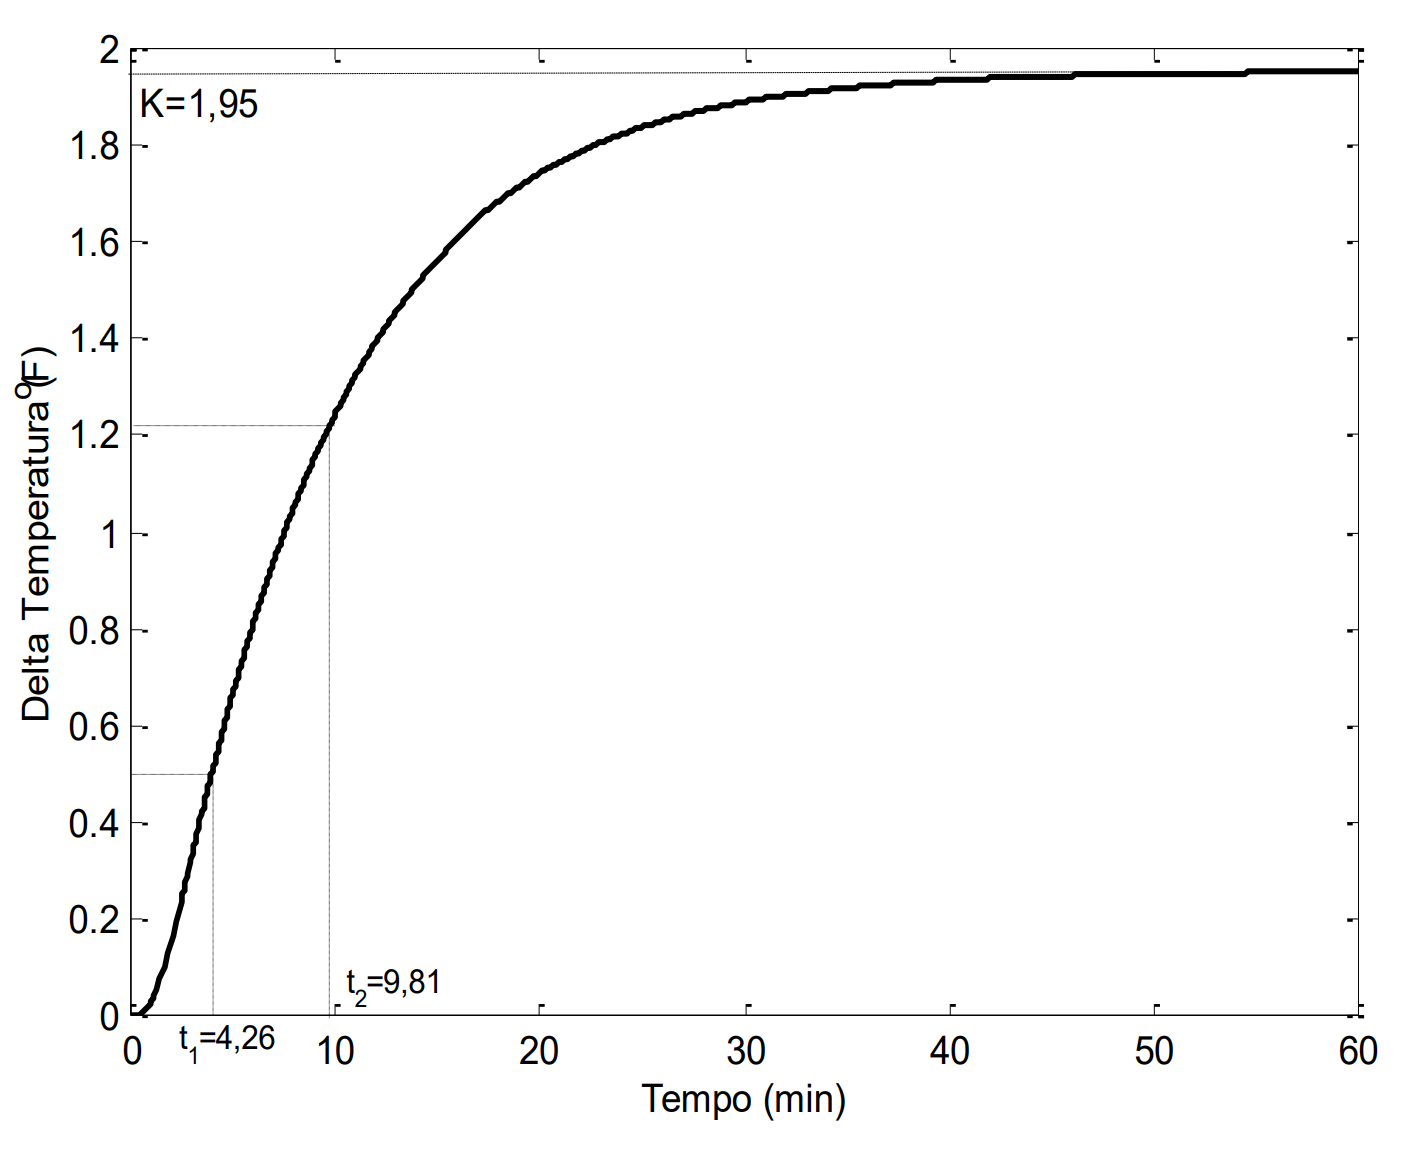
\includegraphics[scale=0.4]{figuras/bib_comp_1_graph}
    \label{fig:bib_comp_1_graph}
    \\
    \vspace{0cm}\hspace{0cm}\small{Fonte: \cite{apostpidsint}}
\end{figure}

\begin{equation}
    \label{eq:bib_comp_1_id}
    \tau = \frac{3}{2}(t_2 - t_1) = 8,33min \;\;,\;\; \theta = t_2 - T = 1,48min \;\;,\;\; K=1,95
\end{equation}

\begin{equation}
    \label{eq:bib_comp_1_model}
    G(s) = \frac{1,95}{8.33 s + 1}e^{-1,48 s}
\end{equation}

\begin{table}[h]
    \begin{center}
        \begin{tabular}{ | l | c | c | c | }
            \hline
            {}                         & {$K_P$} & {$T_I$}   & {$T_D$}   \\
            \hline
            {\textbf{Ziegler-Nichols}} & {3,46}  & {2,96min} & {0,74min} \\
            \hline
            {\textbf{Cohen-Coon}}      & {3,97}  & {3,39min} & {0,52min} \\
            \hline
        \end{tabular}
        \caption{ Métodos da curva de reação para o tanque aquecido}
        \vspace{0cm}\hspace{0cm}\small{Fonte: \cite{apostpidsint}}
        \label{tab:bib_comp_1_restb}
    \end{center}
\end{table}

Para comparação, pode-se instanciar um objeto de modelo com FirstOrderModel, utilizando os mesmos parâmetros fornecidos,
e então utilizar os métodos de aproximação de Ziegler e Nichols e de Cohen e Coon, como é disposto no trecho de código
a seguir:
\begin{lstlisting}[label={lst:bib_comp_1_code1}]
import auto_control_tools as act

model = act.FirstOrderModel(K=1.95, tau=8.33, theta=1.48)

model.view.print_tf()
model.view.print_model_step_response_data()
model.view.plot_model_step_response_graph()

controller = act.ZieglerNicholsControllerAproximation.get_controller(model, act.PID)

controller.view.print_tf()
controller.view.print_controller_step_response_data()
controller.view.plot_controller_step_response_graph()

controller = act.CohenCoonControllerAproximation.get_controller(model, act.PID)

controller.view.print_tf()
controller.view.print_controller_step_response_data()
controller.view.plot_controller_step_response_graph()
\end{lstlisting}

A execução de \ref{lst:bib_comp_1_code1} gera o resultado apresentado em \ref{lst:bib_comp_1_code1_out}
e os gráficos das figuras \ref{fig:bib_comp_1_code1_out_fig1}, \ref{fig:bib_comp_1_code1_out_fig2} e
\ref{fig:bib_comp_1_code1_out_fig3}.

\begin{lstlisting}[label={lst:bib_comp_1_code1_out}]
1.95*exp(-1.48*s)/(8.33*s + 1.0)
{'Overshoot': 0,
 'Peak': 1.9476708568782817,
 'PeakTime': 57.541601473921176,
 'RiseTime': 18.302321365061147,
 'SettlingMax': 1.95,
 'SettlingMin': 1.755565040374366,
 'SettlingTime': 34.082117580267,
 'SteadyStateValue': 1.95,
 'Undershoot': 0.38160197607648316}
1.95*(2.56307692307692*s + 3.46361746361746 + 1.1701410350059/s)*exp(-1.48*s)/((1 + 1.95*(2.56307692307692*s + 3.46361746361746 + 1.1701410350059/s)*exp(-1.48*s)/(8.33*s + 1.0))*(8.33*s + 1.0))
{'Kd': 2.563076923076923,
 'Ki': 1.1701410350058998,
 'Kp': 3.4636174636174637,
 'Overshoot': 8.369513829384001,
 'Peak': 1.08369513829384,
 'PeakTime': 7.7288758064631535,
 'RiseTime': 3.948447422867046,
 'SettlingMax': 1.08369513829384,
 'SettlingMin': 0.900405905739516,
 'SettlingTime': 12.825453331014943,
 'SteadyStateValue': 1.0,
 'Undershoot': 37.50000000000001}
1.95*(2.07319868112764*s + 3.97666897666898 + 1.17187743876933/s)*exp(-1.48*s)/((1 + 1.95*(2.07319868112764*s + 3.97666897666898 + 1.17187743876933/s)*exp(-1.48*s)/(8.33*s + 1.0))*(8.33*s + 1.0))
{'Kd': 2.073198681127638,
 'Ki': 1.1718774387693307,
 'Kp': 3.9766689766689765,
 'Overshoot': 6.845750381802541,
 'Peak': 1.0684575038180253,
 'PeakTime': 7.255513442274729,
 'RiseTime': 3.725804200087023,
 'SettlingMax': 1.0684575038180253,
 'SettlingMin': 0.9034279684915225,
 'SettlingTime': 12.269941651414406,
 'SteadyStateValue': 0.9999999999999999,
 'Undershoot': 32.67455930152555}
\end{lstlisting}



\begin{figure}[H]
    \centering
    \caption{Comparação de resultados - Bibliografia 1 - Gráfico do modelo}
    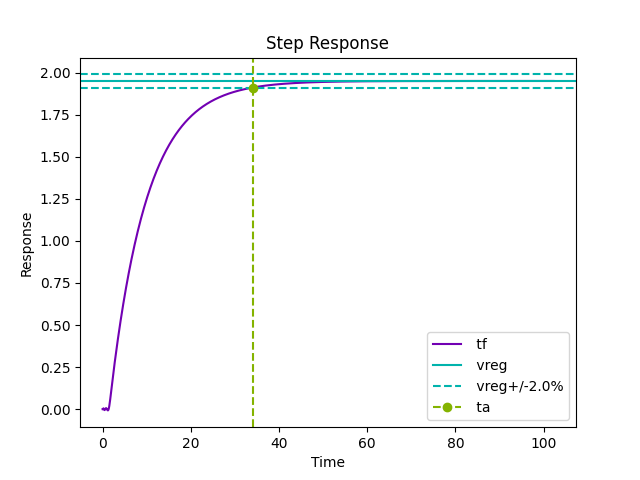
\includegraphics[scale=0.8]{figuras/bib_comp_1_code1_out_fig1}
    \label{fig:bib_comp_1_code1_out_fig1}
    \\
    \vspace{0cm}\hspace{0cm}\small{Fonte: Do autor}
\end{figure}
\begin{figure}[H]
    \centering
    \caption{Comparação de resultados - Bibliografia 1 - Gráfico Ziegler Nichols}
    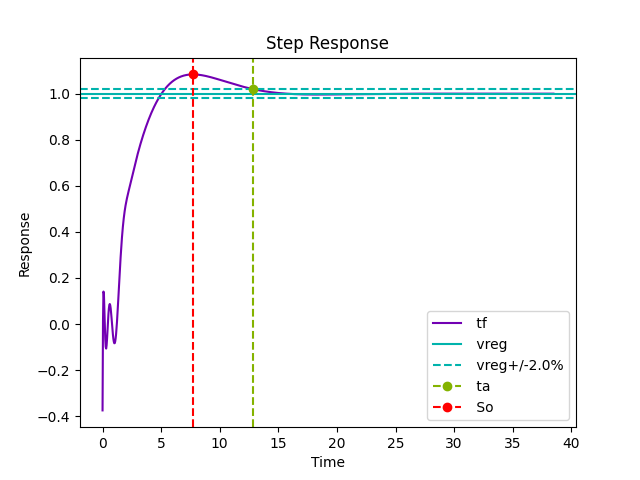
\includegraphics[scale=0.8]{figuras/bib_comp_1_code1_out_fig2}
    \label{fig:bib_comp_1_code1_out_fig2}
    \\
    \vspace{0cm}\hspace{0cm}\small{Fonte: Do autor}
\end{figure}
\begin{figure}[H]
    \centering
    \caption{Comparação de resultados - Bibliografia 1 - Gráfico Cohen Coon}
    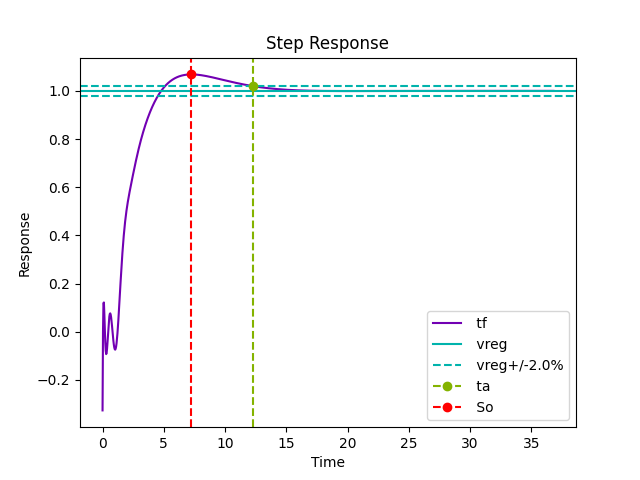
\includegraphics[scale=0.8]{figuras/bib_comp_1_code1_out_fig3}
    \label{fig:bib_comp_1_code1_out_fig3}
    \\
    \vspace{0cm}\hspace{0cm}\small{Fonte: Do autor}
\end{figure}

Calculando $T_I$ e $T_D$ de acordo com a equação \ref{eq:titd}, podemos verificar que os resultados das aproximações de
ganhos concordam com a bibliográfica, conforme detalha a tabela \ref{tab:bib_comp_1_pid_comp}.

\begin{equation}
    \label{eq:titd}
    Ki = \frac{Kp}{Ti} \;\; , \;\; Kd = Kp \times Td
\end{equation}

\begin{table}[h]
    \begin{center}
        \begin{tabular}{ | l | c | c | c | }
            \hline
            {}                         & {$K_P$} & {$T_I$}   & {$T_D$}   \\
            \hline
            {\textbf{Ziegler-Nichols}} & {3,46}  & {2,96min} & {0,74min} \\
            \hline
            {\textbf{Cohen-Coon}}      & {3,97}  & {3,39min} & {0,52min} \\
            \hline
            {\textbf{Ziegler-Nichols Biblioteca}} & {3.4636174636174637}  & {2,96} & {0,74} \\
            \hline
            {\textbf{Cohen-Coon Biblioteca}}      & {3.9766689766689765}  & {3.39341713144} & {0.52134052225} \\
            \hline
        \end{tabular}
        \caption{ Métodos da curva de reação para o tanque aquecido}
        \vspace{0cm}\hspace{0cm}\small{Fonte: Do autor}
        \label{tab:bib_comp_1_pid_comp}
    \end{center}
\end{table}

Contudo, ao comparar os gráficos \ref{fig:bib_comp_1_code1_out_fig2} e \ref{fig:bib_comp_1_code1_out_fig3} com as
respostas apresentadas na figura \ref{fig:bib_comp_1_ctrl_fig},
nota-se uma ligeira diferença no sobressinal entre o gráfico da biblioteca e da bibliografia.
Foram feitos testes em outros sistemas, tentando reproduzir o resultado da bibliografia, contudo apenas resultados
idênticos ao apresentado pela biblioteca foram observados.

\begin{figure}[H]
    \centering
    \caption{Comparação de resultados - Bibliografia 1 - Gráfico Cohen Coon}
    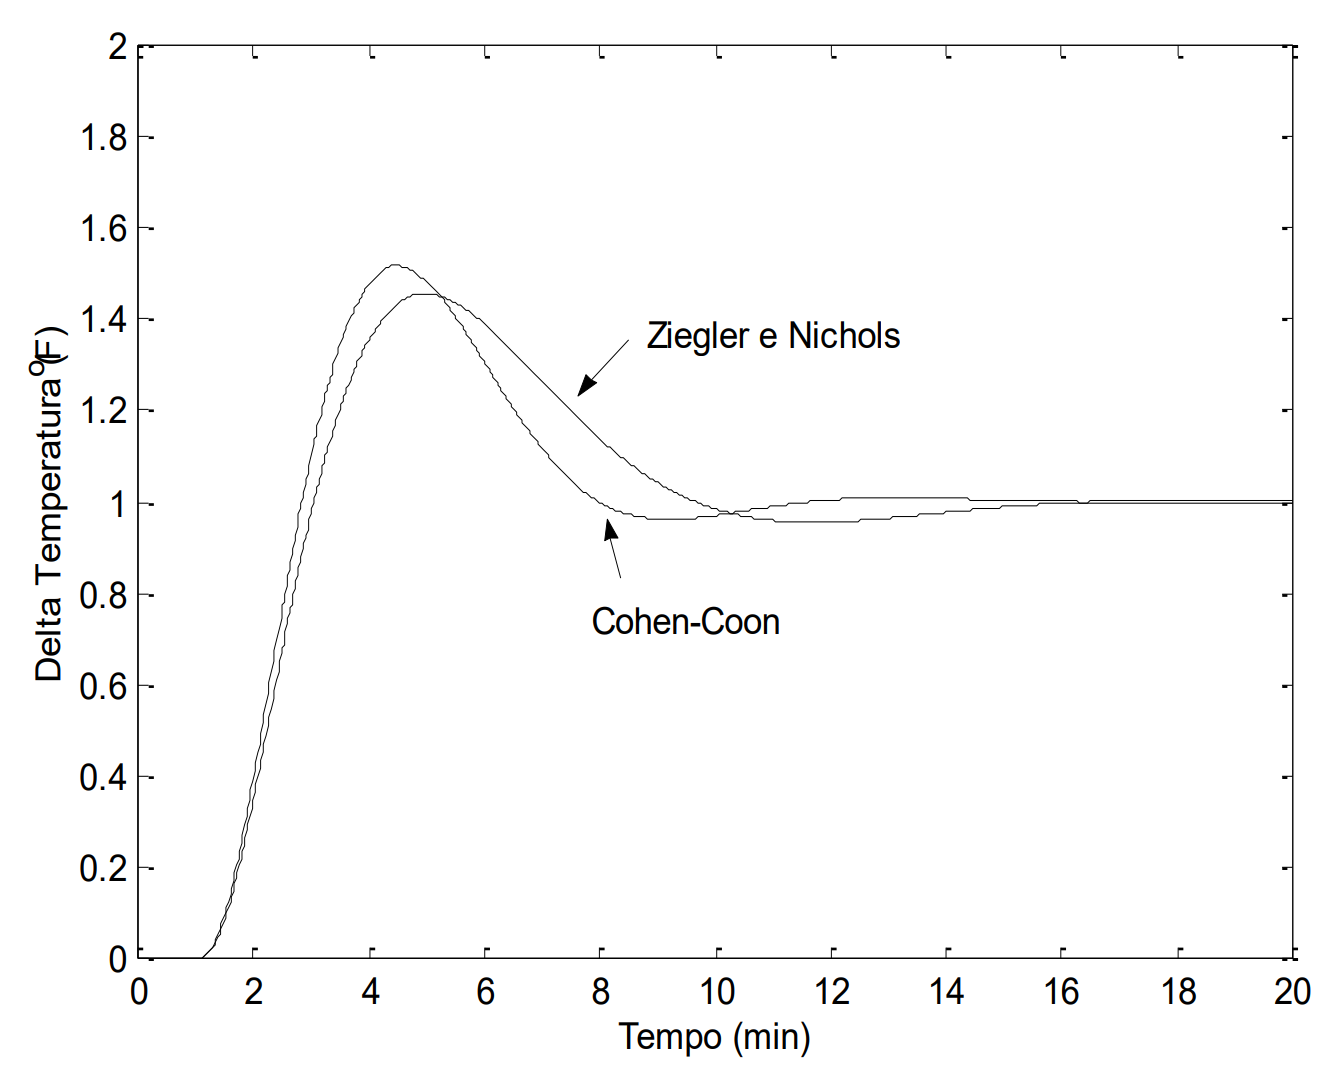
\includegraphics[scale=0.4]{figuras/bib_comp_1_ctrl_fig}
    \label{fig:bib_comp_1_ctrl_fig}
    \\
    \vspace{0cm}\hspace{0cm}\small{Fonte: Do autor}
\end{figure}

\subsection{Biblioteca versus Bishop}

TODO: Pegar caso do bishop e comparar


\section{Comaprações com Experimentos Anteriores}

Para de validar os resultados obtidos, foram pegos dados já existentes de resposta a sinal degrau de algumas plantas
didáticas do laboratório de controle do Campus do IFSC.
Optou-se por fazer o processo de identificação utilizando o método Smith e a aproximação de ganhos de controlador
com o método Cohen Coon.

As plantas trabalhadas são um forno, uma mesa giratória e o nível de um tanque.
Detalhes sobre variáveis manipulada e controlada foram abstraídos por não serem o foco da comparação.
As plantas trabalhadas, em geral, possuíam resposta rápida, com atraso baixo ou nulo, o que, em alguns casos,
impossibilitou o uso do método de Cohen e Coon. Os resultados das identificações e controladores podem ser observados
nas tabelas \ref{tab:results_forno}, \ref{tab:results_mesa}, \ref{tab:results_tanque}.


Não foram recebidas informações sobre os modelos e ganhos obtidos pelos universitários que estavam trabalhando na plata.


\begin{table}[!htbp]
\caption{Resultados obtidos - Forno}
\centering
\begin{tabular}{|c|c|c|c|c|c|c|}
\hline
\textbf{Setpoint} & \textbf{Modelo} & \textbf{Kp} & \textbf{Ki} & \textbf{Kd} & \textbf{Identificação} & \textbf{Malha fechada} \\
\hline
15\% & $\frac{18.08 e^{-22.5s}}{1144.5s + 1.0}$ & 3.76 & 0.068 & 30.70 & 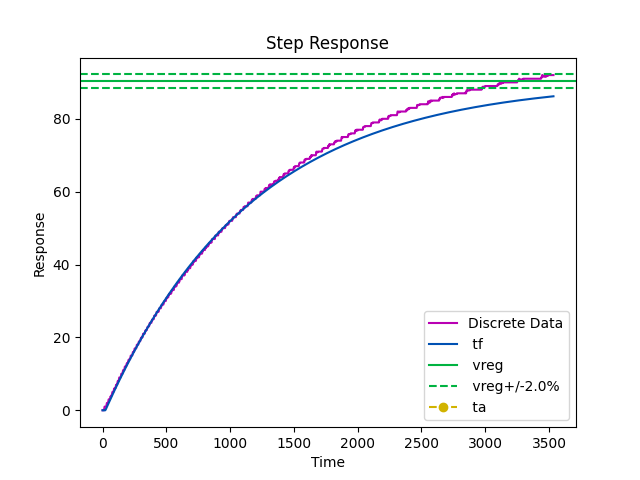
\includegraphics[width=0.2\linewidth]{figuras/forno_15} & 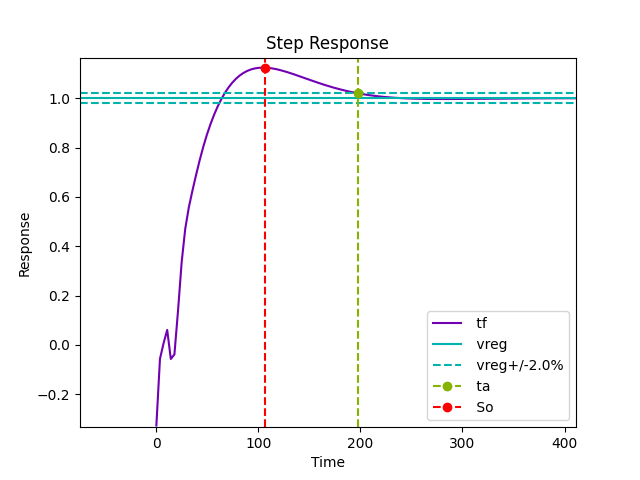
\includegraphics[width=0.2\linewidth]{figuras/forno_15c} \\
\hline
20\% & $\frac{6.90 e^{-19.5s}}{919.5s + 1.0}$ & 9.14 & 0.192 & 64.57 & 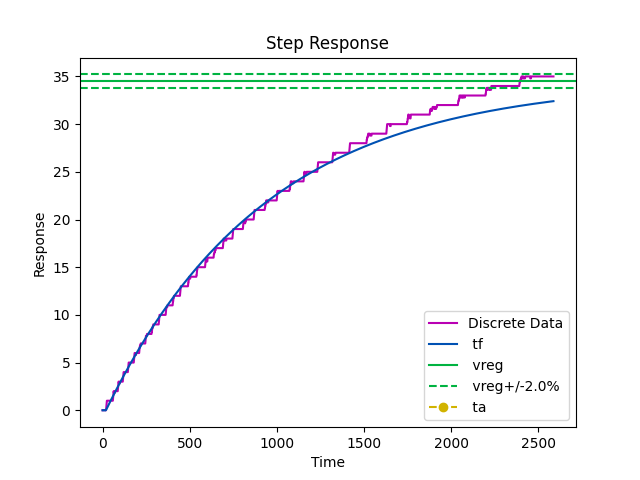
\includegraphics[width=0.2\linewidth]{figuras/forno_20} & 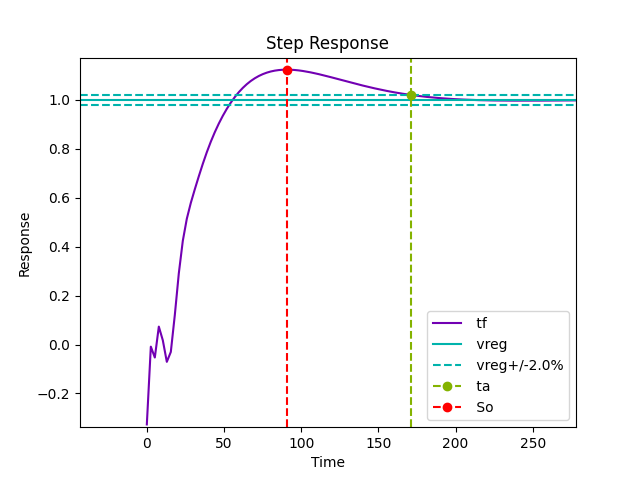
\includegraphics[width=0.2\linewidth]{figuras/forno_20c} \\
\hline
25\% & $\frac{6.68 e^{-17.5s}}{997.5s + 1.0}$ & 11.42 & 0.267 & 72.41 & 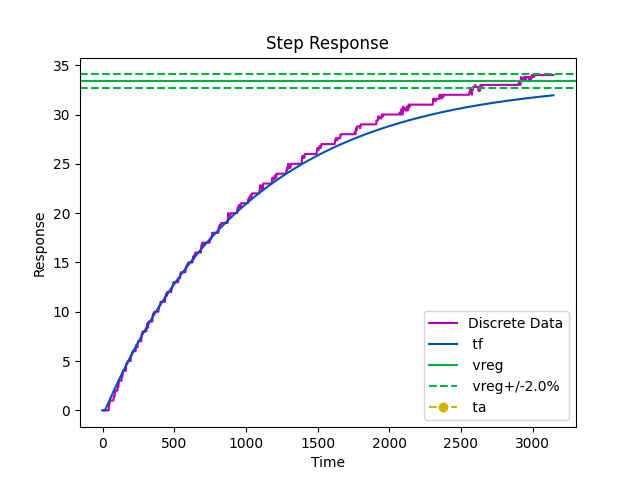
\includegraphics[width=0.2\linewidth]{figuras/forno_25} & 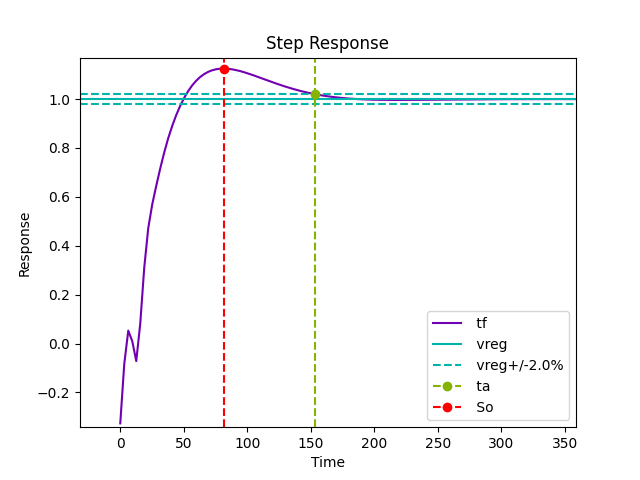
\includegraphics[width=0.2\linewidth]{figuras/forno_25c} \\
\hline
\end{tabular}
\label{tab:results_forno}
\vspace{0cm}\hspace{0cm}\small{Fonte: Do autor}
\end{table}

\begin{table}[!htbp]
\caption{Resultados obtidos - Mesa Giratória}
\centering
\begin{tabular}{|c|c|c|c|c|c|c|}
\hline
\textbf{Setpoint} & \textbf{Modelo} & \textbf{Kp} & \textbf{Ki} & \textbf{Kd} & \textbf{Identificação} & \textbf{Malha fechada} \\
\hline
Mesa (5-10\%) & $\frac{25.93 e^{-1.5s}}{52.5s + 1.0}$ & 1.81 & 0.496 & 0.982 & 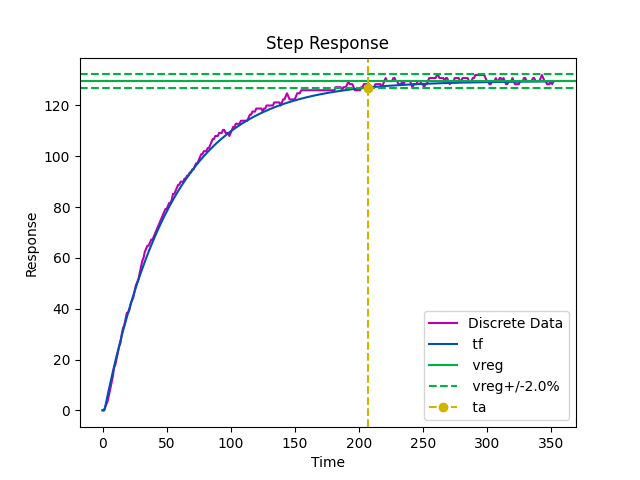
\includegraphics[width=0.2\linewidth]{figuras/mesa_5_10} & 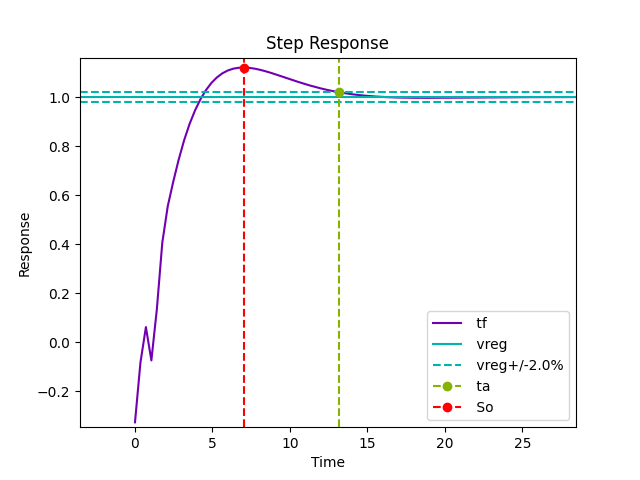
\includegraphics[width=0.2\linewidth]{figuras/mesa_5_10c} \\
\hline
Mesa (10-15\%) & $\frac{17.81 e^{-3.5s}}{40.5s + 1.0}$ & 0.88 & 0.106 & 1.10 & 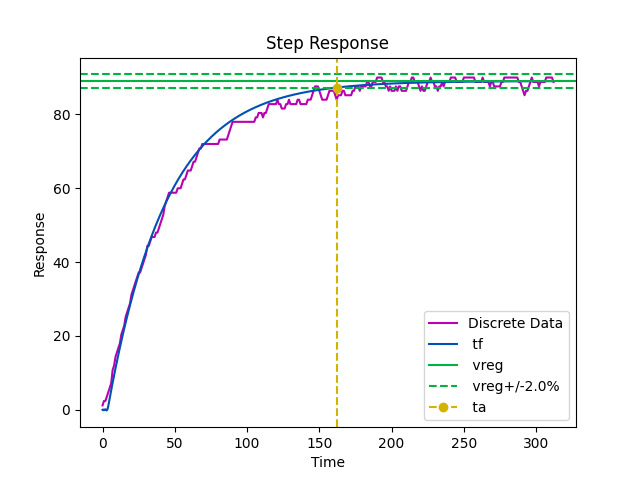
\includegraphics[width=0.2\linewidth]{figuras/mesa_10_15} & 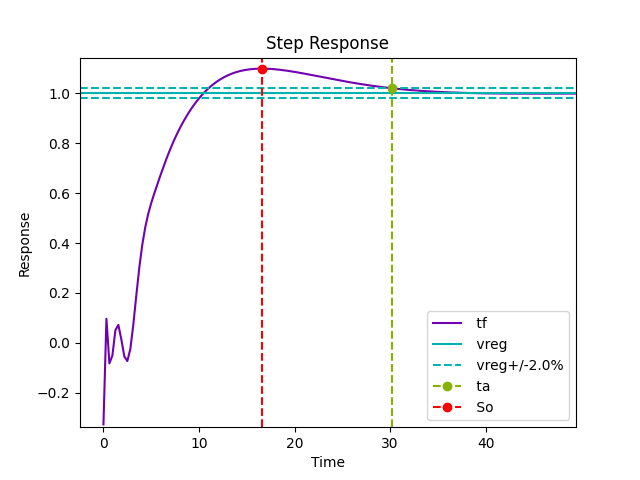
\includegraphics[width=0.2\linewidth]{figuras/mesa_10_15c} \\
\hline
Mesa (15-17\%) & $\frac{15.3}{54.0s + 1.0}$ & - & - & - & 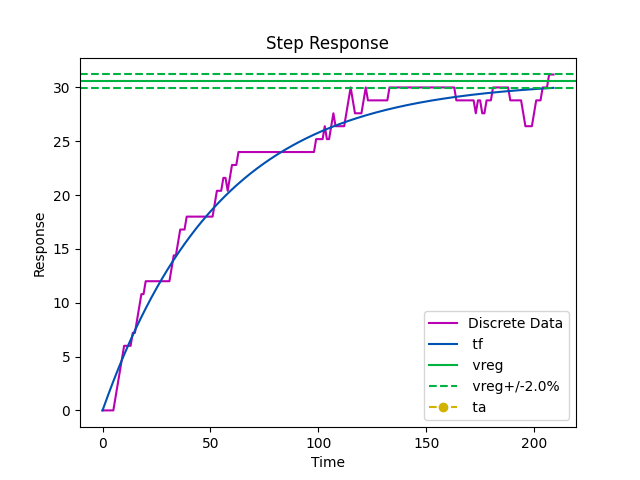
\includegraphics[width=0.2\linewidth]{figuras/mesa_15_17} & \textbf{Sem Atraso} \\
\hline
Mesa (17-20\%) & $\frac{12.0}{37.5s + 1.0}$ & - & - & - & 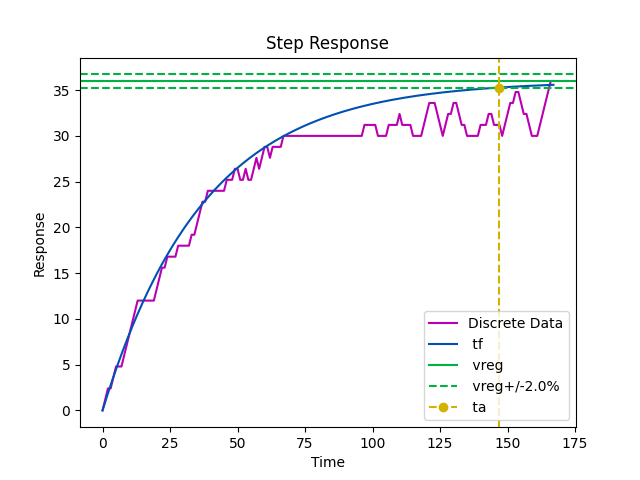
\includegraphics[width=0.2\linewidth]{figuras/mesa_17_20} & \textbf{Sem Atraso} \\
\hline
\end{tabular}
\label{tab:results_mesa}
\vspace{0cm}\hspace{0cm}\small{Fonte: Do autor}
\end{table}

\begin{table}[!htbp]
\caption{Resultados obtidos - Nível Tanque}
\centering
\begin{tabular}{|c|c|c|c|c|c|c|}
\hline
Tanque (40-50\%) & $\frac{2.58 e^{-2.0s}}{18.0s + 1.0}$ & 4.75 & 1.01 & 3.38 & 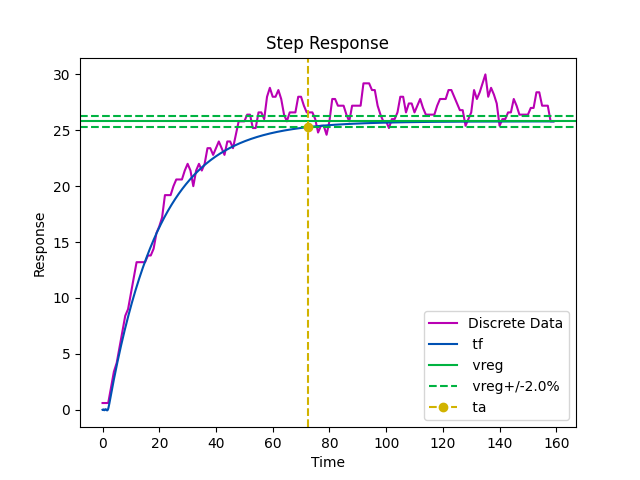
\includegraphics[width=0.2\linewidth]{figuras/tanque_40_50} & 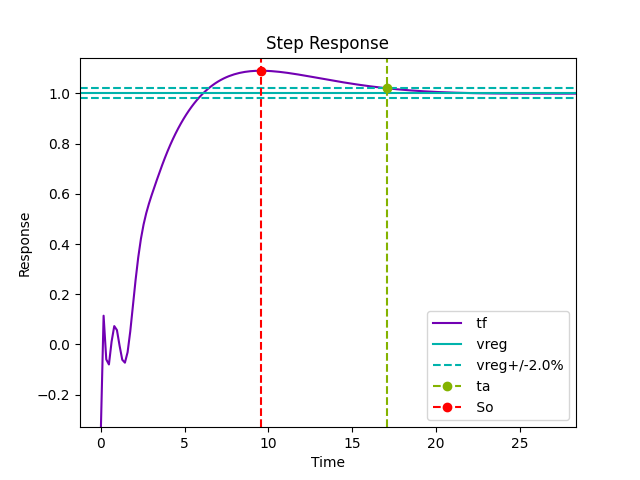
\includegraphics[width=0.2\linewidth]{figuras/tanque_40_50c} \\
\hline
Tanque (40-50\%) & $\frac{3.77 e^{-1.0s}}{33.0s + 1.0}$ & 11.73 & 4.83 & 4.24 & 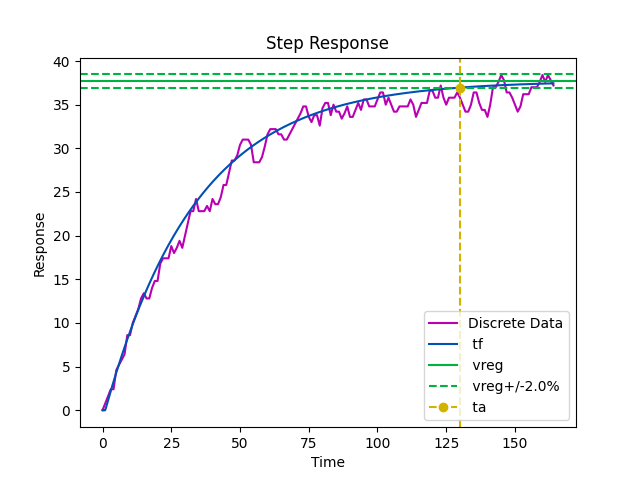
\includegraphics[width=0.2\linewidth]{figuras/tanque_50_60} & 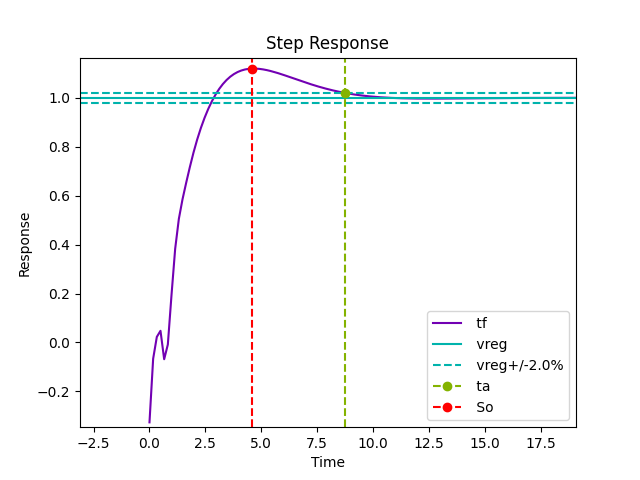
\includegraphics[width=0.2\linewidth]{figuras/tanque_50_60c} \\
\hline
Tanque (40-50\%) & $\frac{3.45}{52.5s + 1.0}$ & - & - & - & 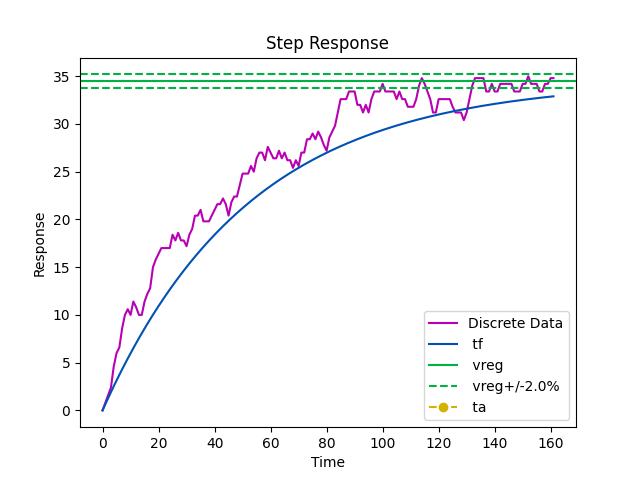
\includegraphics[width=0.2\linewidth]{figuras/tanque_60_70} & \textbf{Sem Atraso} \\
\hline
Tanque (40-50\%) & $\frac{1.26 e^{-5.0s}}{6.0s + 1.0}$ & 1.47 & 0.156 & 2.32 & 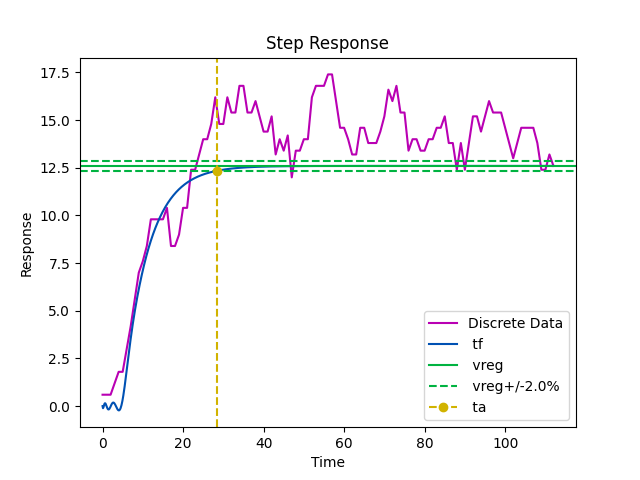
\includegraphics[width=0.2\linewidth]{figuras/tanque_70_80} & 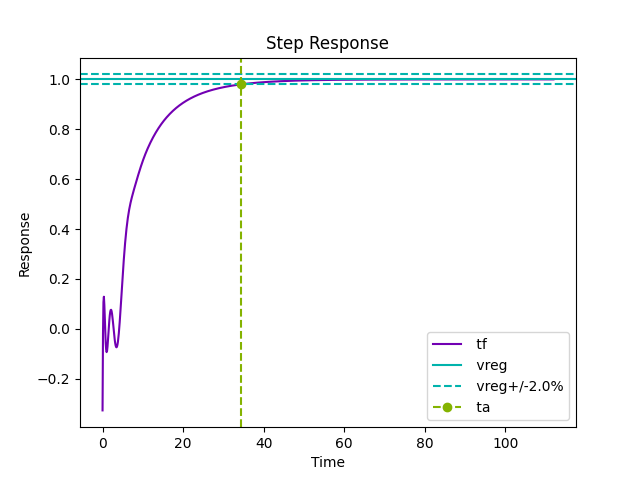
\includegraphics[width=0.2\linewidth]{figuras/tanque_70_80c} \\
\hline
\end{tabular}
\label{tab:results_tanque}
\vspace{0cm}\hspace{0cm}\small{Fonte: Do autor}
\end{table}




\section{Aplicação em Sistema Real}

Ainda não ocorreu
